\scanpage{310}
1) $\uline{\mathrm{Pic}}^\tau$ \uline{fermé} ds $\uline{\mathrm{Pic}}$ ? OK si $f$ est \uline{normal} \deleted{\unsure{universellement} \illegible{1}}

2) $\uline{\mathrm{Pic}}^\tau$ plat sur $S$ ?
\margin{\uline{Non} [contre-exemple de Mumford...]}
\deleted{\unsure{univ. ouvert sur $S$ ?}}

3) $\uline{\mathrm{Pic}}^\tau$ \unsure{univ$^t$} ouvert sur $S$ ?
\margin{\uline{si $f$ normal,} [Vrai, \unsure{en les pts} \deleted{\unsure{dont la}} \inserted{\unsure{de} $\unsure{\tau}$} torsion est première aux car. rés. \unsure{?} OK. en car. $0$]}

4) \deleted{\unsure{4}} La multiplication par $n$ dans $\uline{\mathrm{Pic}}$ (ou dans \deleted{\unsure{$\uline{\mathrm{Pic}}^\tau$ est de type fini}} $\uline{\mathrm{Pic}}^\tau$) est-elle \uline{univ. ouverte} ? (Voir N.b) ?
\inserted{\unsure{pour $n$ ``qcq''}}
\margin{\unsure{expliciter}}
[Oui si $n$ premier aux car. résiduelles; une réponse affirmative à 4), \deleted{pour tt} dans $\uline{\mathrm{Pic}}^\tau$, pour \uuline{tt} $n$, implique une réponse affirmative à 3]
\margin{La multiplication par $n$ est-elle de type fini ?}

\margin{N.B. Soit $G$ un préschéma en groupes sur $S$, tel que les $G_s^\tau$ soient propres, plus gén. \unsure{sans} comp. additives. Alors $G^\tau\to S$ est univ$^t$ ouvert en les pts dont l'ordre de torsion est premier aux car. résiduelles [ $\Longleftarrow$ si $n$ premier aux car. résiduelles, le morphisme $G\xrightarrow{n}G$ est \uuline{étale} ]}

5) $\uline{\mathrm{Pic}}^\tau$ \uline{de type fini sur $S$} $(\Leftrightarrow)$ propre sur $S$
\margin{\uuline{Oui}}
[Si $f$ \deleted{\unsure{normal}}\inserted{\unsure{lisse}}, celà implique $\uline{\mathrm{Pic}}^\tau$ \uline{projectif} sur $S$, j'ignore s'il en est de $\unsure{\overline{=}}$ si $f$ est normal ...]

\unsure{5'}) Une réponse affirmative à 3) en implique une à 5), \deleted{\unsure{dans tous les cas}} \uline{si} $f$ \uline{normal}

OK si les \deleted{$\unsure{\mathrm{NS}}_{\unsure{X_s/k(s)}}$}\inserted{$X_s/k(s)$} ``sans torsion''

\margin{Non, exemple}
\figure{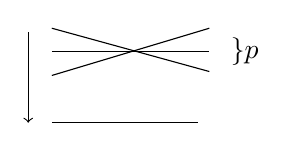
\begin{tikzpicture}[x=1cm,y=1cm]
\draw (0,.65)--(2,.1);\draw (0,.35)--(2,.35);\draw (0,.05)--(2,.65);
\node at (2.45,.35) {$\}p$};
\draw[->](-.3,.6)--(-.3,-.55);\draw (0,-.55)--(1.85,-.55);
\end{tikzpicture}}
\margin{La multiplication par un multiple de $p$ est \unsure{surjective} \illegible{2} \unsure{ouverte} (?) \unsure{comp. irréductibles}}

6) $\uline{\mathrm{Pic}}^\tau$ \deleted{\unsure{est}} n'a-t-il qu'un nb fini de \unsure{$S$-points d'ordre $n$}. \unsure{Non}
\[
[(\uline{\mathrm{Pic}}^\tau_{X/S}\text{ de type fini}\Longleftrightarrow\uline{\mathrm{Pic}}^\tau_{X'/S'}\text{ n'a qu'un nb fini de comp. irréductibles \unsure{au dessus|en dehors} d'un ouvert \unsure{non vide convenable|dense de $S'$ constructible}, }\forall S'\text{ fermé irréductible de }S.
\]

7) $\unsure{\mathrm{rang}}(\mathrm{NS})$ reste-t-il majoré ?
\margin{\uuline{oui}}

8) \deleted{\unsure{$\uline{\mathrm{Pic}}^\tau$ est de type fini sur}}
Les composantes connexes de $\uline{\mathrm{Pic}}_{X/S}$ sont elles de type fini sur $S$ ??
\margin{\uuline{non}}
$\uline{\mathrm{Pic}}_{X/S}$ est-il réunion disjointe \deleted{\unsure{par}}\inserted{de} $\uline{\mathrm{Pic}}^\tau_{X/S}$ ?
\margin{$\unsure{\overline M}$ la réponse à 5) ne semble \unsure{pas aussi évidente ici|pas asymptotiquement liée} .... \unsure{d'invariants} \uline{\unsure{stables|étales}}}

9) Définition de $\uline{\mathrm{Pic}}_{X/k}/\uline{\mathrm{Pic}}^\tau_{X/k}$ ...

\figure{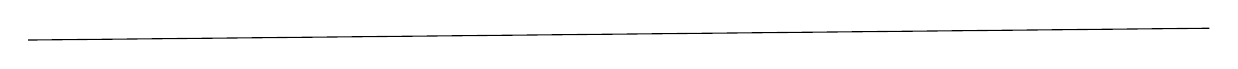
\begin{tikzpicture}\draw (0,0)--(15,.15);\end{tikzpicture}}
\uline{Howard} $\left\{\begin{array}{l}\text{Multiplicité de }\uline{\mathrm{Pic}}^\tau\\ \circledast\ \text{Compatibilité aux spécialisations ???}\end{array}\right.$
\margin{$\circledast$ Questions liées à la \unsure{platitude|flèche}}
\margin{$\circledast$ Questions d'existence et descente....}

\figure{\begin{tikzpicture}[x=1cm,y=1cm]
\draw[->,double] (0,5.3)--(0,4.7);
\draw[<->,double](-.25,4.4)..controls(-.55,3.8)and(-.5,2.8)..(-.25,2.2);
\draw[<->,double](0,1.4)--(0,0);
\draw[->,double](.3,-.35)--(.3,-1.15);
\draw[->](1.5,4.1)..controls(2.2,3.9)and(2.1,1)..(4.1,.9);
\draw[<->](3.4,4.4)--(4.1,4.9);
\end{tikzpicture}}
\figure{\begin{tikzpicture}[x=1cm,y=1cm]
\draw (1.8,8.1) ellipse (.26 and .22);
\draw (1.55,7.99) -- (1.3,7.8);
\draw (.9,6.9) ellipse (.72 and .13);
\draw (-.65,6.45) ellipse (.35 and .18);
\draw[->](-.4,6.7)--(-.7,6.25);
\draw (-1.1,5.3) .. controls (-1.35,5.5) and (-1.1,5.9) .. (-.8,5.95) .. controls (.1,6.2) and (.35,5.55) .. (-.2,5.25) .. controls (-.55,5.05) and (-.9,5.13) .. (-1.1,5.3);
\draw (-.95,4.5) ellipse (.35 and .22);
\draw (2.8,3.15) .. controls (3.7,3.22) and (4.4,3.2) .. (4.9,3.13) -- (5,1.4) .. controls (5.1,.75) and (4.7,.8) .. (4.35,.8) -- (2.65,.84) .. controls (2.25,.9) and (2.3,1.2) .. (2.4,1.6) -- (2.8,3.15);
\draw (4.55,.85) .. controls (4.7,.6) and (5.1,.55) .. (5.18,.82);
\draw (-1.25,.15) ellipse (.3 and .17);
\draw (-1.12,-.55) ellipse (.36 and .2);
\draw (-.85,7.65) .. controls (-.65,7.25) and (-.72,6.9) .. (-.8,6.6);
\draw (-.89,7.67) .. controls (-.7,7.25) and (-.77,6.9) .. (-.85,6.61);
\end{tikzpicture}}
\mspage{309}
